% !TeX spellcheck = en_US
\addscenariosection{1}{Clash Scenario}{Secret Bomb Stash}{\images/implosion.png}

\begin{multicols}{2}

\textbf{Author:} NeuroN

\textbf{Source:} \href{https://discord.com/channels/740870068178649108/1278750250722525203/1278750250722525203}{Archon Studios Discord}

\textit{Rumors speak of an abandoned bomb stash in this area.
Use it to destroy your opponents.
But be careful -- your enemies might already be one step ahead.}

\subsection*{\MakeUppercase{Scenario Length}}
This Scenario is played over 8 Rounds, with up to 4 additional tie-breaking Rounds if needed.

\subsection*{\MakeUppercase{Player Setup}}
\textbf{Player Count:} 2--4, 6 Player FFA or 2vs2, 2vs2vs2, 3vs3 Alliance

\textbf{Starting Resources:} 40 \svg{gold}

\textbf{Starting Income:} 20 \svg{gold}, 2 \svg{building_materials}, 1 \svg{valuables}

\textbf{Starting Units:}
\begin{itemize}
  \item 2 × A Few \svgunit{bronze} Units with the lowest Recruitment cost
  \item A Few \svgunit{silver} Units with the lowest Recruitment cost
\end{itemize}

\textbf{Town Buildings:} \svgunit{bronze} Dwelling, \svgunit{silver} Dwelling, Citadel, Mage Guild

\textbf{Map Tile Pool:} None

\textbf{Additional Bonus} (replaces Starting Bonus):

\begin{itemize}
  \item Search (4) the Artifact Deck and shuffle the Card into your M\&M Deck.
\end{itemize}
Before the start of the Scenario, instead of performing the usual Search (2) Spells twice, each player performs a Search (4) Spells once.
\textbf{Players start at Level III} (before the start of the Scenario, instead of the usual Search (2) Abilities twice, each player performs a Search (4) Abilities once).

\subsection*{\MakeUppercase{Map Setup}}
\begin{itemize}
  \item Center (VI--VII) Map Tile \textbf{must contain the Grail Field}.
  \item Each Near Tile \textbf{must contain an Obelisk} (if that's not possible, treat Witch Huts as Obelisks).
  \item Take the following Map Tiles and arrange them as shown in the Scenario map layout ($\boldsymbol{P}$ stands for the number of players):
\end{itemize}

\textbf{For a 2- and 4-player Scenario:}
\begin{itemize}
  \item $\boldsymbol{P}$ × Starting (I) Map Tile
  \item 4 × Near (IV--V) Map Tile
  \item 1 × Center (VI--VII) Map Tile
\end{itemize}

\textbf{For a 3- and 6-player Scenario:}
\begin{itemize}
  \item $\boldsymbol{P}$ × Starting (I) Map Tile
  \item 6 × Near (IV--V) Map Tile
  \item 1 × Center (VI--VII) Map Tile
\end{itemize}

\subsection*{\MakeUppercase{Victory Conditions}}

Deposit bombs (Grail) into the enemy Town to score Victory Points (VPs).
The game lasts for 8 Rounds:
\begin{itemize}
  \item A player/alliance wins when they score 3 VPs. The Scenario ends immediately after a single player/alliance deposits their third bomb.
  \item If no one scores 3 VPs by the end of the 8th Round, the player/alliance with the most VPs wins the Scenario.
  \item If VPs are tied, the Scenario goes into sudden death. The first player/alliance to score a VP during the next 4 Rounds (9--12) wins the Scenario.
  \newpage
  \item In any other situation, the game ends in a tie between the players with the most VPs.
\end{itemize}

\subsection*{\MakeUppercase{Defeat Conditions}}
Players lose if they don't score enough VPs within the designated number of Rurns.

\subsection*{\MakeUppercase{Timed Events}}

\textbf{Every Astrologers Proclaim Round:}
\begin{itemize}
  \item Each Hero gains +1 \svgeven{movement}, except for the current bomb carrier.
\end{itemize}

\subsection*{\MakeUppercase{Additional Rules}}

During this Scenario:

\begin{itemize}
  \item Heroes cannot attack other players' Towns unless they are carrying the bomb.
  \item Heroes cannot attack the bomb carrier from their Starting Town Field.
  \item In Clash Mode with more than 2 players, the Town that was bombed most recently cannot be bombed again.
\end{itemize}

\textbf{Center Tile:}

\begin{itemize}
  \item On the Center Tile, players can freely move through neutral combats of Level VI, as if they had the basic Pathfinding Ability (they can choose to fight there but don't have to, and cannot end their turn there without resolving the combat).
  \item Level VII combat is ignored. The Hero that reaches the Grail space receives the bomb (Grail token). Place the Grail token under the bomb-carrying Hero's miniature.
\end{itemize}

\textbf{The Bomb:}

\begin{itemize}
  \item The bomb carrier cannot gain extra \svgeven{movement} from any Card, Town Building, Map Location, or any other effect.
  \item If your other Hero or an allied Hero is adjacent to the bomb carrier, you can transfer the bomb to them.
  \item If defeated, the bomb is placed on the space where the Hero was defeated and can be claimed by any other Hero by visiting that Field.

  \item If held by the Main Hero:
  \begin{itemize}
    \item If defeated, the Hero does not have to pay their opponent 10 \svg{gold}, nor do they gain \svg{morale_negative}.
  \end{itemize}

  \item If held by a Secondary Hero:
  \begin{itemize}
    \item If defeated, the Hero is moved to the Town instead of being removed.
    \item The Hero can use your M\&M Deck during combat.
  \end{itemize}
\end{itemize}

\textbf{Obelisks:}

\begin{itemize}
  \item When first flagged, the Hero gains +1 \svgeven{movement}.
  \item On each visit (including the first), you can choose to either:
  \begin{itemize}
    \item Move the visiting Hero to any other Obelisk already flagged by you (if that Obelisk is occupied by another Hero, your Hero cannot move there).
    \item If the Hero carries the bomb, transfer the bomb to your other Hero (or any allied Heroes).
  \end{itemize}
\end{itemize}

\textbf{Scoring Victory Points (VPs):}

A player/alliance earns 1 VP after winning a siege or entering the enemy Town while carrying the bomb.
\begin{itemize}
  \item After such an event, the victorious Hero is moved back to their own Town, and the Grail token is returned to the Grail space in the center. If any Hero is standing on that Field when the Grail is placed, they immediately become the bomb carrier.
  \item The defending player does not lose control of their Town after losing the siege.
\end{itemize}

You can track VPs by collecting Faction Cubes of your opponent's color or using a color not in use by any player.

\end{multicols}

\newpage

\begin{tikzpicture}[overlay]
  \centering
  \node at (4.5, -4) {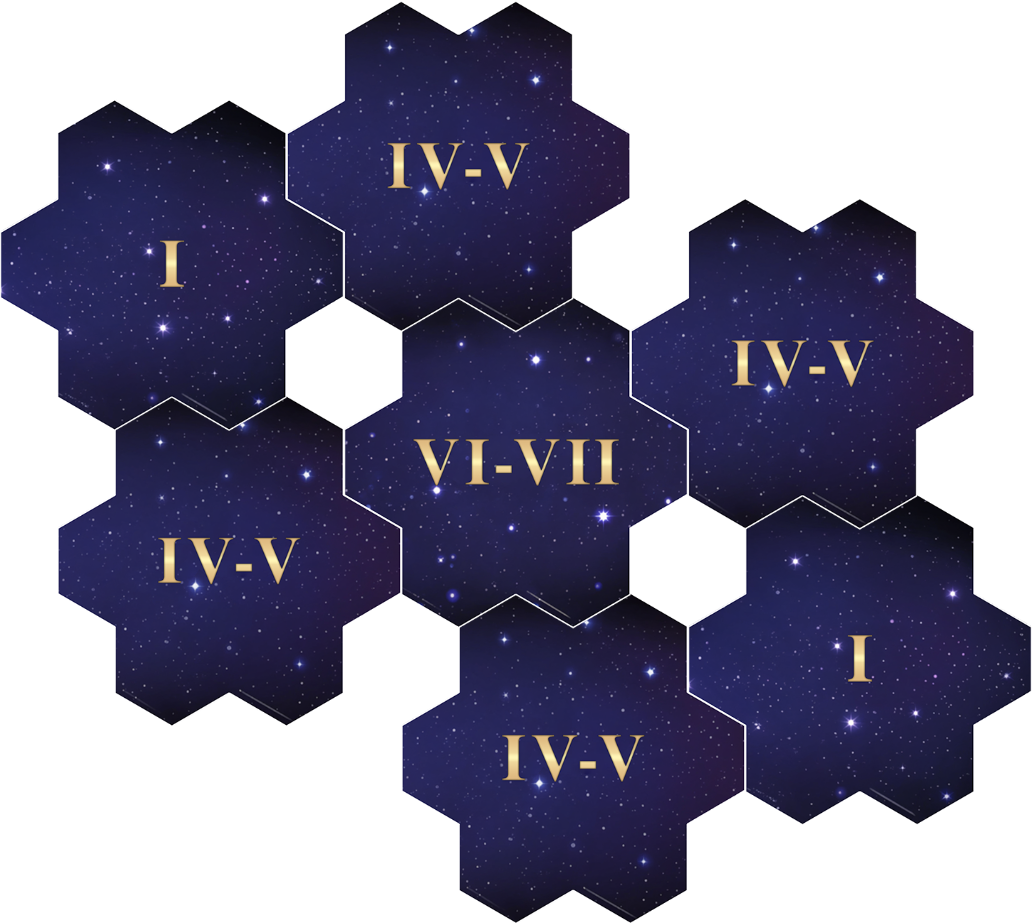
\includegraphics[scale=0.2]{\maps/secret-bomb-stash-2p.png}};
  \node at (4.5, -8) {\footnotesize{\textbf{\MakeUppercase{2-PLAYER SCENARIO}}}};
  \node at (13.5, -4) {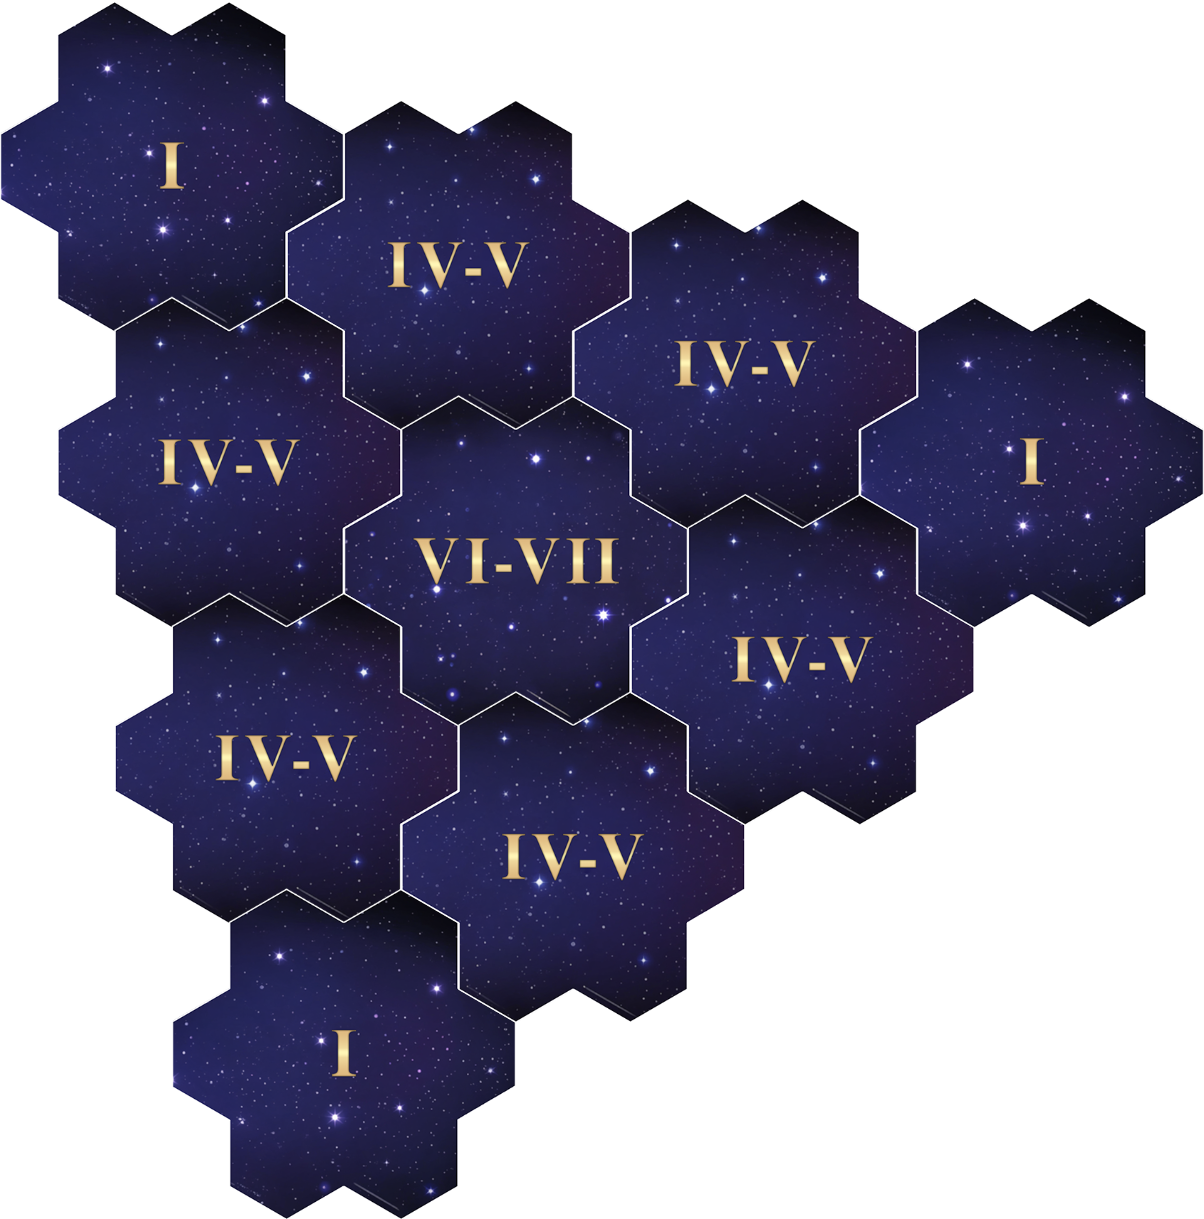
\includegraphics[scale=0.2]{\maps/secret-bomb-stash-3p.png}};
  \node at (13.5, -9) {\footnotesize{\textbf{\MakeUppercase{3-PLAYER SCENARIO}}}};
  \node at (4, -17) {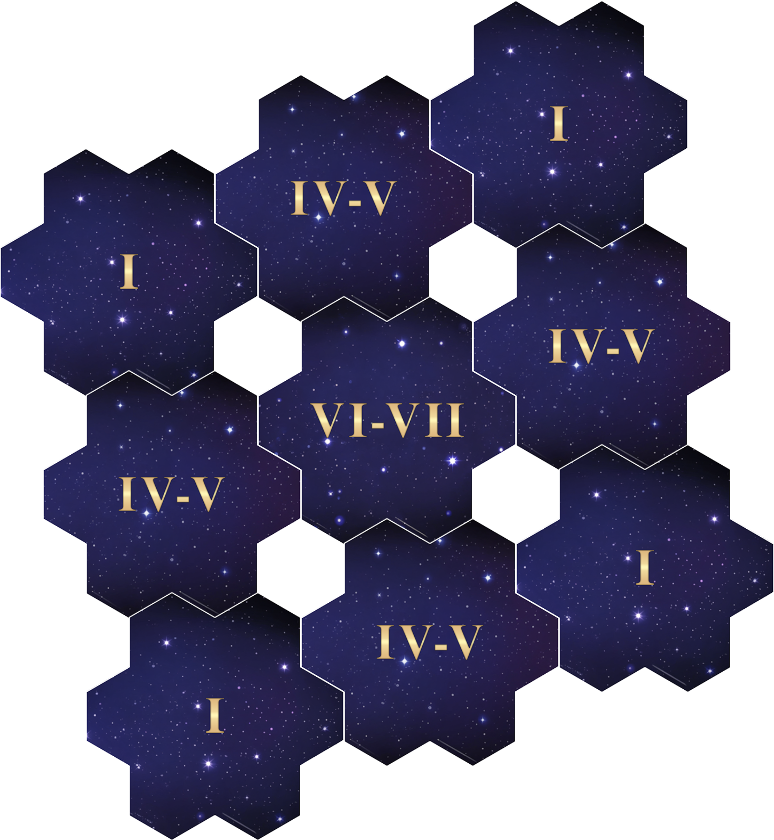
\includegraphics[scale=0.2]{\maps/secret-bomb-stash-4p.png}};
  \node at (5.5, -21.5) {\footnotesize{\textbf{\MakeUppercase{4-PLAYER SCENARIO}}}};
  \node at (13, -16) {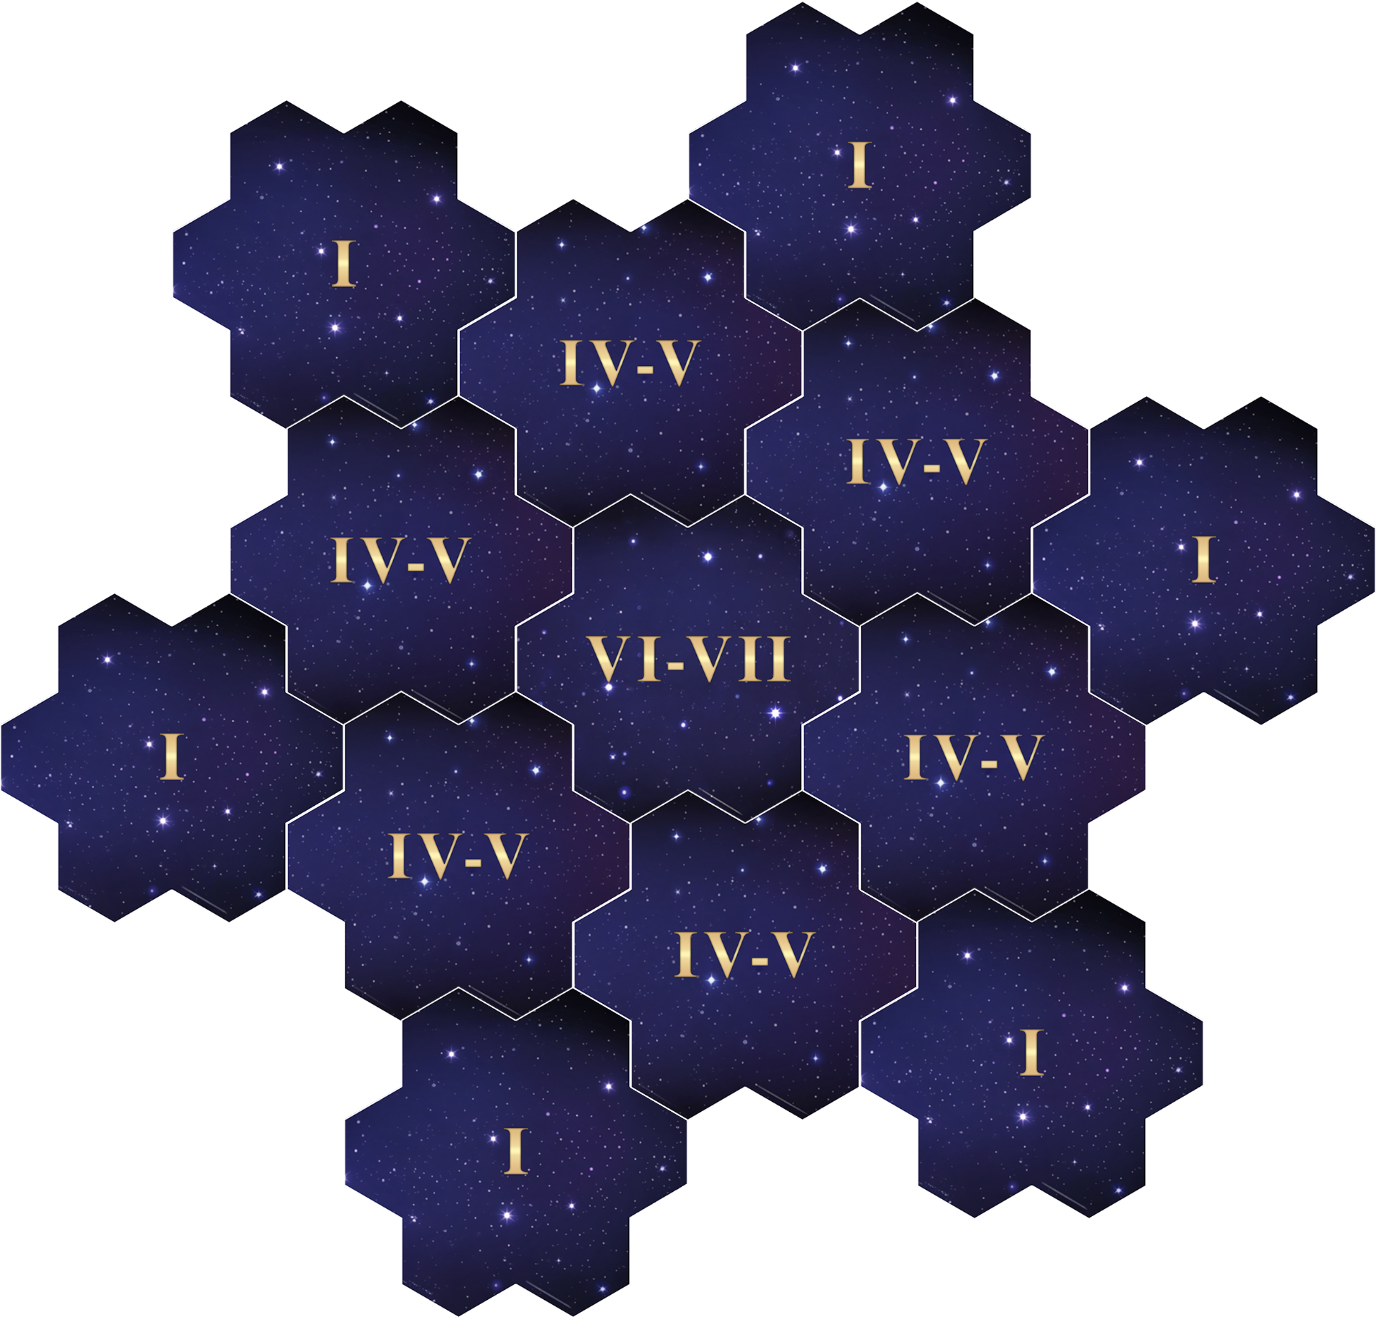
\includegraphics[scale=0.2]{\maps/secret-bomb-stash-6p.png}};
  \node at (13, -21.5) {\footnotesize{\textbf{\MakeUppercase{6-PLAYER SCENARIO}}}};
\end{tikzpicture}
